\documentclass[11pt]{standalone}
\usepackage[usenames]{color} %used for font color
\usepackage{amssymb} %maths
\usepackage{amsmath} %maths

\usepackage[no-math]{fontspec}
\usepackage{unicode-math}
\setmainfont{Lato}
\setmathfont{Stix Two Math}

\usepackage{pgf,xcolor}
\definecolor{itwm_blue_04}{HTML}{005A94}
\definecolor{itwm_red}{HTML}{C00000}
\definecolor{itwm_yellow}{HTML}{FFEC7F}

\usepackage{tikz}
\usetikzlibrary{shapes.misc, shadows, decorations, arrows}
\usetikzlibrary{backgrounds}
\usetikzlibrary{calc}
\usepackage{pgfplots}
\pgfplotsset{compat=newest}
\usepgfplotslibrary{fillbetween}
\usepackage{tikzpagenodes}
\usetikzlibrary{patterns}


\begin{document}
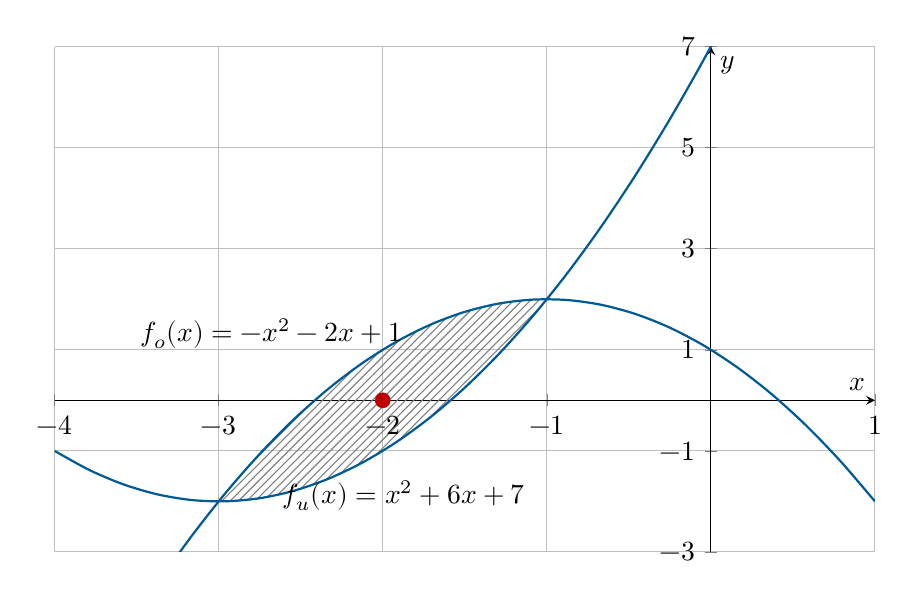
\begin{tikzpicture}
\begin{axis}[
    domain=-4:1,
    axis lines = center,
    xlabel = {$x$},
    ylabel = {$y$},
    height=8cm, width=12cm, 
    xmin=-4, xmax=1, ymin=-3, ymax=7,
    ytick={-3,-1,...,7},
    xtick={-4,-3,...,1},
    grid = both
]
\addplot[draw=itwm_blue_04, domain=-4:1, smooth, thick, name path=g]{-x^2-2*x+1} node [pos=0.6, above, left] {$f_o(x)=-x^2-2x+1$};
\addplot[draw=itwm_blue_04, domain=-4:1, smooth, thick, name path=f]{x^2+6*x+7} node [pos=0.1, below, right] {$f_u(x)=x^2+6x+7$};
\addplot[pattern=north east lines, pattern color=gray] fill between [of=f and g, soft clip={domain=-3:-1}];

\node[fill, itwm_red, circle,inner sep=-2] at (-2,0) {};
%\draw [->, thick] (-1, -1) -- (-0.2,0) {};
%\node [below] at (-1, -1) {$f_u(x)=0$};
%\draw [->, thick] (1.5, 1.2) -- (0.5,0.5) {};
%\node [above] at (1.5, 1.2) {$f_o(x)=-x+1$};

\end{axis}
\end{tikzpicture}
\end{document}

